\externaldocument{../3/chapter_modeling}
\externaldocument{../5/chapter_implementation}
\externaldocument{../appendix/chapter_app}
\startchapter{Communication Analysis}
\label{chapter:alo}
I defined a message transferring communication between two programs in Chapter \ref{chapter:mod}. The goal of this research is to develop a method to identify the communications from a dual\_trace. A dual\_trace is a pair of assembly-level execution traces of two interacting programs. In this chapter, I discuss the characteristics of the assembly-level execution trace, and then I formalize the dual\_trace. For all the traces that comply with this abstract dual\_trace formalization, the analysis approach presented in this chapter can be applied.


The process of the communication analysis is shown in Figure \ref{overview}. It takes the two traces in the dual\_trace as input and outputs the identified communications. In this overview figure, there are four components. The function call event reconstruction component will analyze the traces and try to reconstruct all function calls of the functions in the functions descriptor. These two sequences of events of these two traces will then flow into the stream extraction component separately. In each event sequence, the events might be triggered by different endpoints of different communications. I consider all the events triggered by the same endpoint as a stream. The stream extraction component will extract two sets of streams. After that, the stream matching component will take both of the stream sets as input and try to match them by their channel identifiers and output the potential identified communications. Finally, the data verification component will verify each communication and see if it satisfy the communication content preservation. Algorithms are designed separately for each component. Details about each elements and components of this overall process will be discussed in the following sections.


\begin{figure}[H]
\centerline{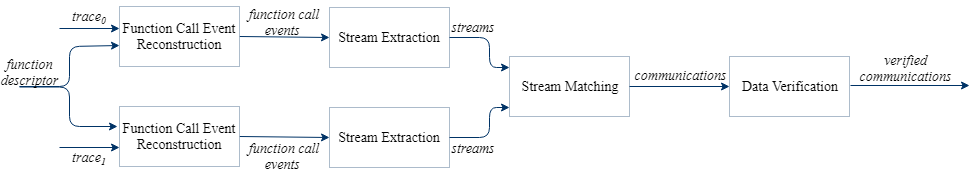
\includegraphics[scale=0.5]{Figures/overview}}
\caption{Process of the communication analysis through a dual\_trace}
\label{overview}
\end{figure}

\section{Dual\_Trace}\label{dualtrace}
In this section, I formalize a dual\_trace. All traces aligning with this formalization can be used as the input of the analysis process shown in Figure \ref{overview}. A dual\_trace consists of two assembly-level execution traces of two interacting programs. There is no timing information of these two traces which means we don't know the timing relationship of the events of one trace with respect to the other. However, the captured instructions in a trace are ordered in execution sequence. 

A dual\_trace is formalized as :

$dual\_trace = \lbrace trace_0, trace_1\rbrace$

where $trace_0$ and $trace_1$ are two assembly-level execution traces.

An execution trace consists of a sequence of instruction lines and can be defined as: 

$ trace = (l_1, l_2, ..., l_n)$ 

Each instruction line contains the executed instruction, the changed memory, the changed registers and the execution information and can be defined as a tuple:

$l = <ins, mch, rch, exetype, syscallInfo>$

where $ins$ is the instruction, $mch$ is the memory changes, $rch$ is the register changes, $exetype$ is the execution type which can be instruction, system call entry, and system call exit, $syscallInfo = <exeName, funcName>$ only appears when $exetype$ is system call entry or system call exit. $exeName$ is the executable file name (e.g., .dll and .exe), while $funcName$ is the name of a system function in this executable file.

Figure \ref{tracedefined} is an example of a piece of execution trace complying with the definition of a trace. 

\begin{figure}[H]
\centerline{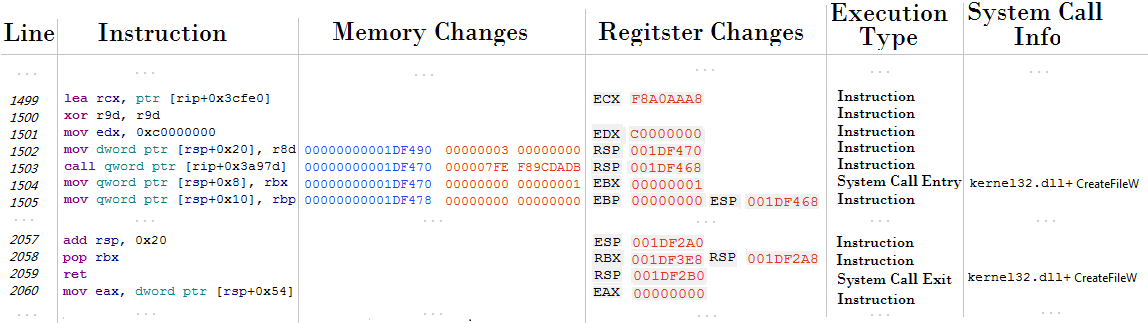
\includegraphics[scale=0.5]{Figures/tracedefined}}
\caption{An example trace }
\label{tracedefined}
\end{figure}



\section{Functions Descriptors}\label{cdesc}
There could be lots of function calls in an execution trace. However, most of them are not of interest. I am only concerned with the function call events of a specific communication method, such as TCP, UDP, and Named Pipe. To be able to identify and reconstruct the function calls, I define a functions descriptor as:

$cdesc = \lbrace fdesc_1, fdesc_2,...,fdesc_p \rbrace$

Each element, $fdesc$, is a function description and can be defined as:

$fdesc = < name, type, inparamdesc, outparamdesc >$

where, $name$ is the function name, $type$ is the function type which can be one of the four types: $open$, $close$, $send$ and $receive$. $inparamdesc$ is the input parameter descriptions illustrating how the registers and memory contents map to a list of parameters of interest (you might not care for all parameters of a function) of a given function call, and $outparamdesc$ is the output parameter descriptions similar to the input parameter descriptions. 

Table \ref{functionexample} is an example of a function description. In this example, the function name is $ReadFile$, it is a function for data receiving, so its function type is $receive$. The input parameter description has one concerned parameter, $Handle$, while the output parameter description has two parameters, ${RecvBuffer}$ and $MessageLength$. $Handle$ is a parameter which is a value stored in the register RCX. The $RecvBuffer$ is an address for the input message stored in the register RAX. The $MessageLength$ is a output value stored in register R9. The value of the input parameters can be retrieved from the memory state on the function call instruction line, while the value of the output parameters can be retrieved from the memory state on the function return instruction line. If a parameter is an address instead of a value, the address should be retrieved first, then the retrieved address should be used to find the buffer content in the memory state. The function description requires the understanding of the calling convention of the operating system. The Microsoft x64 calling convention can be found in Appendix \ref{convention}. More examples of communication method descriptions will be given in Chapter \ref{chapter:newsol}.

\begin{table}[H]
        \centering
        \caption{An example of a function description}
        \label{functionexample}
        \begin{tabular}{|l|l|l|l|l|l|l|l|}
            \hline
             \multirow{2}{*}{{\textbf{Name}}} & \multirow{2}{*}{{\textbf{Type}}} & \multicolumn{3}{c|}{\textbf{Input Parameter Description}} & \multicolumn{3}{c|}{\textbf{Output Parameter Description}} \\
              \cline{3-8} 
             & & \textbf{Name}& \textbf{Register} &  \textbf{Addr/Val} & \textbf{Name}& \textbf{Register} &  \textbf{Addr/Val}  \\
             \hline
             \multirow{2}{*}{ReadFile}
             &\multirow{2}{*}{receive} &  \multirow{2}{*}{Handle} & \multirow{2}{*}{RCX} & \multirow{2}{*}{Value} & RecvBuffer & RDX  & Addr\\
              \cline{6-8} 
             & & & & & MessageLength & R9  & Val\\
            \hline            
        \end{tabular}
    \end{table}

\section{Function Call Event Reconstruction Algorithm}
In last two sections, I formalized the assembly-level execution trace and defined the functions descriptor of a communication method. The functions descriptor helps to locate the function calls and retrieve the parameters of interest from an execution trace. These function calls contain the information of a communication, such as the channel identifier, the packets sent or received, etc. Before any communication can be identified, the function calls of that communication method have to be reconstructed first. 

In this section, I define the function call event and present an algorithm to reconstruct the function call events from an assembly-level execution trace. 

With the functions descriptor and the execution trace as input, the function call event reconstruction algorithm identifies the function call entry instruction line and reconstructs the input parameters from the memory state of that line. Then it identifies the function call exit line of the corresponding function call and reconstructs the output parameters from the memory state of the function exit line. After iterating through the whole execution trace, the algorithm outputs a sequence of function call events of length $m$. This sequence of events can be defined as $etr$:

$etr = (ev_1, ev_2, ..., ev_m)$

A function call event $ev$ in $etr$ is defined as a tuple:

$ev = <funN, inparams, outparams, type>$

where $funN$ is the function name, $inparas$ includes all the input parameters with the parameter name and value, $outparas$ includes all the output parameters, and $type$ is the event type which is inherited from the function description and can be one of the four types: $open$, $send$, $receive$ and $close$.


If the parameter is an address, the parameter's value is the string from the buffer pointed to by that address instead of the buffer address.

Algorithm \ref{eventAlg} presents the pseudocode for the function call event reconstruction algorithm. This algorithm is designed to reconstruct the function call events for one communication method. If multiple communication methods are being investigated, this algorithm can be run multiple times to analyze each of them. Since there are usually a small number of functions of interest for a communication method compared to the number of instruction lines in the execution trace, the time complexity of this algorithm is $O(N)$ and $N$ is the number of instruction lines in the trace.

\begin{algorithm}[H]
\DontPrintSemicolon
\caption{{\bf Function Event Reconstruction Algorithm} \label{eventAlg}}
\tcc{$trace$ is the assembly-level execution trace with a sequence of instruction lines: $(l_1, l_2, ..., l_n)$, $cdesc$ is the functions descriptor contains a set of function descriptions: $fdesc_1, fdesc_2, ..., fdesc_p$, $etr$ is a sequence of function call events}
\KwIn{ $trace, cdesc$}
\KwOut{$etr$}
$etr \leftarrow \emptyset$\; 
$i \leftarrow 1$\;
\tcc{Emulate the Execute of each instruction line of the trace}
\While{$i \leq n$}{
       $l \leftarrow trace[i]$\;
       $i \leftarrow i+1$\;
       Execute the instruction of $l$\;
     \For{$fdesc \in cdesc$}{
        \If{$l$ is a call to the function described by $fdes$}{
                Create an new function call event $ev$\;
                $ev.funN  \leftarrow fdesc.name$\;
                $ev.type  \leftarrow fdesc.type$\;
                Get the input parameters from the memory state and append them to  $ev.inparams$\;
                $i \leftarrow i+1$\;
                \While{$i \leq n$}{
                      $l \leftarrow trace[i]$\;
                      $i \leftarrow i+1$\;
                      Execute the instruction of $l$\;
                      \If{$l$ is a exit of the function described by $fdes$}{
                          Get the output parameters from the memory state and append them to  $ev.out params$\;
                          Break the inner while loop\;
                      }                     
                }
                $etr.append(ev)$\;
                Break the For loop\;
         }
}
}

\KwRet $etr$\;
\end{algorithm} 

An example of a sequence of function call events as the output of this algorithm is shown in Listing\ref{eventsexample}.

\begin{lstlisting}[caption= Example of  $etr$, label=eventsexample]
{funN:CreateNamedPipe, type:open,inparams:{Handle:18, FileName:mypipe}, outparams:{}},
{funN:CreateNamedPipe, type:open,  inparams:{Handle:27,  FileName:Apipe}, outparams:{}},
{funN:WriteFile, type:send, inparams:{Handle:27, SendBuf:Message1}, outparams:{MessageLen:9}},
{funN:WriteFile, type:send, inparams:{Handle:27, SendBuf:Message2}, outparams:{MessageLen:9}},
{funN:ReadFile, type:receive, inparams:{Handle:27}, outparams:{RecvBuf:Message3, MessageLen:9}},
{funN:CloseHandle, type:close, inparams:{Handle:27}, outparams:{}}
\end{lstlisting}

\section{Channel Open Mechanisms}\label{mecha}
The channel open mechanism affects the stream extraction and stream matching strategy. So I discuss them before presenting those algorithms. The channel open mechanism of a named pipe and message queue is relatively simple. In the Windows implementation, only one function call is related to the handle identification of the stream. However, for TCP and UDP the mechanism is complicated.

In all communication methods, all operations such as packet send and receive use a handle as an identifier to bind them to an endpoint. This handle is generated or returned by a channel open function call and will be assigned to an input parameter for all other related function calls to indicate the corresponding endpoint. However, in other communication methods, the handles might have other names, such as file handle for Named Pipe or socket (sometime called socket handle) for UDP and TCP. All of these are essentially equivalent.

A handle is an unique identifier among all open endpoints. An open endpoint is one that can still be used for data transfer. For example, if there are ten endpoints opened for communications, the handles for all these ten endpoints are different. However, if any of these endpoints is closed, its handle can be reused for other newly created endpoints. Since the handle is the unique identifier for an endpoint and its related events, we need to know it to identify an endpoint and its corresponding function call events. 

Moreover, since two endpoints (one from each trace) are connected to a channel for communication, each endpoint has to know the identifier of the channel to connect to it. This channel identifier is usually given to the endpoint in the channel open function calls. The endpoint will remember this channel and know where the data should be sent to and received from. Therefore, to identify a communication, the channel identifier given to an endpoint needs to be found during the channel open stage.

In the following subsections, I will explain how the different communication methods open their channels for communication.

\subsection{Named Pipe Channel Open Mechanisms} 
In the Named Pipe communication method, a named pipe server is responsible for the creation of the pipe. The creation of a named pipe returns the file handle of that pipe. So on the server side, the identification of the stream needs to identify the pipe creation function call. Clients can connect to the pipe with the pipe name after it is created. So, on the client side, the identification of the stream is to identify the pipe connection function call. The handle returned by the pipe creation and connection function calls will be used later when data is being sent to or received from a specified pipe. In a named pipe, the file is used as the media of the channel, so the identifier in this case is the file name. \cite{WinNamedpipe} Figure \ref{namedpipeopen} exemplifies the channel set up process for a Named Pipe communication in Windows. 

\begin{figure}[H]
\centerline{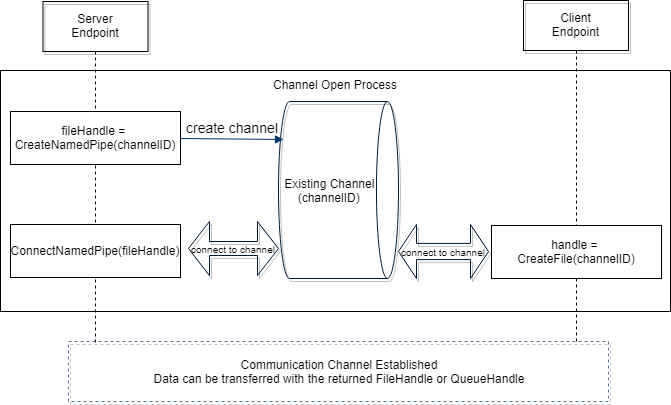
\includegraphics[scale=0.5]{Figures/namepipechannelopen}}
 \caption{Channel open process for a named pipe in Windows}
\label{namedpipeopen}
\end{figure}
    
\subsection{Message Queue Channel Open Mechanisms} 
For the Message Queue communication method, the endpoints of the communication can create the queue or use the existing one. However, both endpoints have to open the queue before accessing it. The handle returned by the open queue function will be used later when messages are being sent or received to indicate the corresponding endpoint. The identifier of the channel is the input for the open queue function. \cite{WinMSMQ} Figure \ref{msmqopen} exemplifies the channel set up process for a Message Queue communication in Windows.

\begin{figure}[H]
\centerline{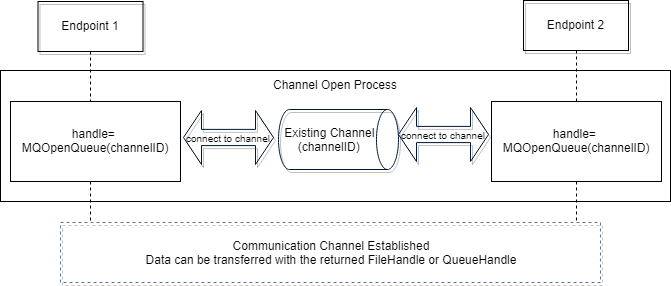
\includegraphics[scale=0.5]{Figures/msmqchannelopen}}
 \caption{Channel open process for a message queue in Windows}
\label{msmqopen}
\end{figure}

\subsection{UDP and TCP Channel Open Mechanisms} 
For the UDP and TCP communication methods, the communication channel is set up by both endpoints. The socket create function should be called on both endpoints. After the socket handles are created, the server endpoint binds the socket to its service address and port by calling the socket bind function. Then the server endpoint calls the listening function to accept the client connection. The client calls the connection function to connect to the server. When the listening function call returns successfully, a new socket handle will be generated and returned for further data transfer between the server endpoint and the connected client endpoint. After all these operations are performed successfully, the channel is established and the data transfer can start. During the channel open stage, server endpoint has two socket handles, the first one is used to listen to the connection from the client, and the second one is used for real data transfer. The server's address and port are considered to be the identifier of the channel \cite{winsock}. Figure \ref{channelopen2} exemplifies the channel open process for TCP and UDP in Windows.
    
\begin{figure}[H]
\centerline{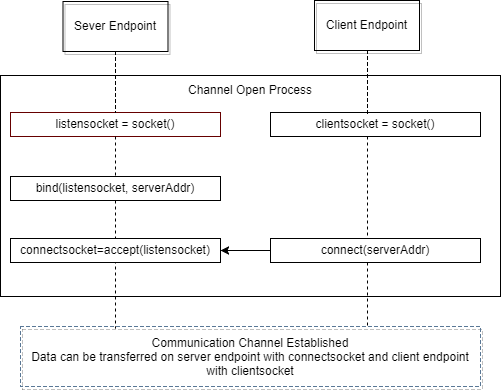
\includegraphics[scale=0.6]{Figures/tcpudpchannelopen}}
 \caption{Channel open model for TCP and UDP in Windows}
\label{channelopen2}    
\end{figure}

\section{Stream Extraction Algorithm}
The sequence of function call events output by the function call event reconstruction algorithm may belong to different endpoints. We need to further separate these events for each endpoint. Each subset of these events belonging to an endpoint is considered to be a stream. There are four types of events in each stream: open, send, receive and close. Hence, we can further divide a stream into substreams which are called open stream, send stream, receive stream, and close stream. There will be only one type of event in each of these streams. The reason to divide a stream into sub streams is that the later stream matching only needs the information extracted from the open stream and the data verification only needs the data extracted from the send and receive streams. So separating them will simplify the later processes. Since a stream corresponds to an endpoint and an endpoint is connected to a channel, it is necessary to know the endpoint handle and the channel identifier corresponding to this stream. 

A stream is formally defined as a tuple:

$s = <handle, channelId, so, ss, sr, sc>$

where $handle$ is the handle of the endpoint, $channelId$ is the identifier of the channel the endpoint of this stream is connected to, $so$ is the open stream, $ss$ is the send stream, $sr$ is the receive stream, $sc$ is the close stream. 

The sub streams $so$, $ss$, $sr$, $sc$ are sequences of events, $sx$ is defined as:

$sx = (ev_1, ev_2, ..., ev_p)$

The event numbering of in this sub stream is different from the original sequence of event. For example, $ev_1$ in $sx$ and $ev_1$ in $etr$ might be different events.

The stream extraction algorithms are designed to separate the streams from a sequence of function call events. In these algorithms, a stream is identified by the endpoint handle output by channel open function calls. Then all other events will be added to this stream.  According to the channel open mechanisms discussed in Section \ref{mecha}, the identifier of the channel and the handle of the endpoint can be retrieved from the channel open function call events.

The input of this algorithm is the sequence of events $etr = (ev_1, ev_2, ..., ev_n)$ from the function call event reconstruction algorithm. Since the events in $etr$ are reconstructed in sequence of the instructions which are ordered by the time of occurrence, the events are implicitly sorted by time of occurrence. 

The outputs of the stream extraction algorithms are a set of streams of size $p$, which can be defined as:

$str = (s_1, s_2, ..., s_p)$

According to the channel open mechanisms, two different algorithms are designed, one for Named Pipe and Message Queue, while the other for TCP and UDP. 

\subsection{Stream Extraction Algorithm for Named Pipe and Message Queue}
This algorithm is designed for the extraction of the streams for Named Pipe and Message Queue. Since for each endpoint of the communication, only one channel open function call is needed to identify the endpoint, it is simple to identify the stream once the endpoint handle is found. 

The same handle may be reused by another endpoint once it is closed by the channel close function call. Therefore, before the detection of the channel close function call, if a new channel open function call with the same returned handle is detected, the second channel open is treated as an error. The error handling is not discussed in this algorithm. This algorithm recognizes this error by having $tempstreams$ to keep track of the streams that are still open. Once the stream is closed, this stream will be removed from $tempstreams$. The time complexity of this algorithm is $O(N)$ , $N$ is the number of events in the trace.

\begin{algorithm}[H]
\DontPrintSemicolon
\caption{{\bf Stream Extraction Algorithm for Named Pipe and Message Queue} \label{streamext1}}
\tcc{$etr$ is a sequence of function call events output by Algorithm \ref{eventAlg}; $str$ is a set of streams corresponding to a set of endpoints}
\KwIn{$etr$}
\KwOut{$str$} 
$str \leftarrow \emptyset$\; 
\tcc{a temporary stream set for all open streams}
$tempstreams \leftarrow \emptyset$\;
\For{$ev \in etr$}{
   \If{$ev.type = open$ }{
         $h \leftarrow$the handle in $ev.outparams$\;
         \If{$tempstreams[h]$ not exist}{
         $tempstreams[h] \leftarrow$ a new $s$\;
         $tempstreams[h].handle \leftarrow h$\;
         $tempstreams[h].channelId \leftarrow$ the channel identifier from $ev.inparams$\; 
         $tempstreams[h].so.append(ev)$\;   
         }
   }
   \ElseIf{$ev.type = send$}{    
   $h \leftarrow$the handle in $ev.inparams$\;  
          \If{$tempstreams[h]$ exist}{
         $tempstreams[h].ss.append(ev)$\;
         }
   }
   \ElseIf{$ev.type = receive$}{    
   $h \leftarrow$ the handle in $ev.inparams$\;  
          \If{$tempstreams[h]$ exist}{
         $tempstreams[h].sr.append(ev)$\;
         }
   }
      \ElseIf{$ev.type = close$}{    
   $h \leftarrow$ the handle in $ev.inparams$\;  
          \If{$tempstreams[h]$ exist}{
         $tempstreams[h].sc.append(ev)$\;
         $str.append(tempstreams[h])$\;        
         remove $tempstreams[h]$ from $tempstreams$\;
         }
   }
   \Else{
    unknown event type error\;
   }       
}
\KwRet $str$\;
\end{algorithm} 

\subsection{Stream Extraction Algorithm for TCP and UDP}
This algorithm is designed for extracting the streams for TCP and UDP. In the channel open stage, socket handles are created by function calls of the socket create function in both client and server. On the server side, this created socket is only used for listening to the client's connection. The listening is accomplished by calling the accept function. One of the input parameters of the accept function call is the listening socket handle, and the output of it is a new data transmission socket handle. 


In this algorithm, each created socket will be identified as a stream. The two socket handles in the server side are considered to be two handles for two streams, the stream identified by the listening handle is called the parent stream and the one identified by the data transmission handle is called the child stream. The events in the parent stream contain the information needed for stream matching algorithm for the child stream later, so the child stream will inherit all the events from its parent. 

Similar to the algorithm for Named Pipe and Message Queue, the reuse of a handle can only happen after a stream identified by this handle is closed. Otherwise the handle reuse will be treated as an error. The error handling is not discussed in this algorithm. A set, $tempstreams$, is also used in this algorithm to check for the open streams.

The time complexity of this algorithm is also $O(N)$, $N$ is the number of events in the trace.

\begin{algorithm}[H]
\caption{{\bf Stream Extraction Algorithm for TCP and UDP} \label{streamext2}}
\tcc{$etr$ is a sequence of function call events output by Algorithm \ref{eventAlg}; $str$ is a sequence of streams corresponding}
\KwIn{$etr$}
\KwOut{$str$} 
$str \leftarrow \emptyset$\; 
\tcc{a temporary stream set for all open streams}
$tempstreams \leftarrow \emptyset$\;
\For{$ev \in etr$}{
   \If{$ev.funN = socket$}{
      $h \leftarrow$ the handle in $ev.outparams$\;
      \If{$tempstreams[h]$ not exist}{
         $tempstreams[h] \leftarrow$ a new $s$\tcp*[f]{a new stream}\;
         $tempstreams[h].handle \leftarrow h$\;
         $tempstreams[h].so.append(ev)$\;
      }     
   }  
   \ElseIf{$ev.funN = bind$ or $ev.funN = connect$}{
      $h \leftarrow$ the handle in $ev.inparams$\;
      \If{$tempstreams[h]$ exist}{
         $tempstreams[h].channelId \leftarrow$ address and port parameter in $ev.inparams$\;
         $tempstreams[h].so.append(ev)$\;
      }     
   }   
   \ElseIf{$ev.funN = accept$}{
      $h \leftarrow$ the handle in $ev.inparams$;\tcp*[f]{the handle of parent stream}\; 
      $hc \leftarrow$ the handle in $ev.outparams$;\tcp*[f]{the handle of child stream}\; 
      \If{$tempstreams[h]$ exist}{  
        \If{$tempstreams[hc]$ not exist}{
            $tempstreams[hc] \leftarrow$ a new $s$;\tcp*[f]{a new stream for the child}\; 
        }
         $tempstreams[hc].handle \leftarrow hc$\;
         $tempstreams[hc].channelId \leftarrow tempstreams[h].channelId$\;
         $tempstreams[hc].so.append(tempstreams[h])$;\tcp*[f]{append parent's events}\;           
         $tempstreams[hc].so.append(ev)$;\tcp*[f]{append the current event}\;  
      }     
   }     
   \ElseIf{$ev.type = send$}{  
      $h \leftarrow$ the handle in $ev.inparams$\;    
      \If{$tempstreams[h]$ exist}{
         $tempstreams[h].ss.append(ev)$\;
      }
   }
   \ElseIf{$ev.type = receive$}{  
      $h \leftarrow$ the handle in $ev.inparams$\;    
      \If{$tempstreams[h]$ exist}{
         $tempstreams[h].sr.append(ev)$\;
      }
   }
   \ElseIf{$ev.type = close$}{
      $h \leftarrow$ the handle identifier from $ev.paras$\;
      \If{$tempstreams[h]$ exist}{
         $tempstreams[h].sc.append(ev)$\;
         $str.append(tempstreams[h])$\;        
         remove $tempstreams[h]$ from $tempstreams$\;
      }
   }      
   \Else{
      unknown event type or name error\;
   }   
}
\KwRet $str$\;
\end{algorithm} 


\section{Stream Matching Algorithm}\label{streammatch}
The function event extraction algorithm and the stream extraction algorithms work on a single execution trace. As defined before, a communication has two endpoints and each endpoint corresponds to a stream. To identify a communication from the dual\_trace, the two streams from that communication need to be found. 

The stream matching algorithm iterates over all the streams extracted from both traces of a dual\_trace and tries to match one stream of a trace to a stream of the other trace using the channel identifier held by each stream.

The channel identifiers held by the streams are retrieved in the stream extraction algorithm and are different for different communication methods. For TCP and UDP, the channel identifier is the server's address and port. For Named Pipe, the channel identifier is the file name, while for Message Queue, the channel identifier is the queue name.  

 The inputs of this algorithm are two sequence of streams $str_0$ and $str_1$ which are output by the stream extraction algorithm. The output of this algorithm is a sequence of the preliminary communications $cs$ of two matched streams. Each matched item in it is a triple $<channelId, s_0, s_1>$, where $channelId$ is the identifier of the channel, while $s_0$ and $s_1$ are the streams from $trace_0$ and $trace_1$ that correspond to the communication performed by each program on that channel. The time complexity of this algorithm is $O(N*M)$, $N$ and $M$ are the number of streams in both traces.
 
 \begin{algorithm}[H]
\DontPrintSemicolon
\caption{{\bf Stream Matching Algorithm for Named Pipe and Message Queue} \label{matchAlg}}
\tcc{$str_0$ and $str_1$ are two sequences of streams from $trace_0$ and $trace_1$. $cs$ is a sequence of preliminary communications}
\KwIn{$str_0, str_1$}
\KwOut{$cs$}
$cs \leftarrow \emptyset$\; 
\For{$s_0 \in str_0$}{
   \For{$s_1 \in str_1$}{     
     \If{$s_0.channelId = s_1.channelId$}{
            Create a new communication $c \leftarrow <channelId, s_0, s_1>$\;
            $cs.append(c)$\; 
      }
   }
}
\KwRet $cs$\;
\end{algorithm} 

This matching algorithm is not fully reliable. There are two situations in which the matching will fail. Take Named Pipe for example, the named pipe server is connected by two clients (client1 and client2) using the same file. The server trace and the client1 trace are analyzed as a dual\_trace, while the server trace and the client2 trace are analyzed as the other dual\_trace. In the server trace, there are two streams found. In each client trace, there is one stream found. For the dual\_trace of the server and client1, there will be two possible identified communications, one is the real communication for server and client1, while the other is an error which actually is for server and client2. The stream in client1's trace will be matched by the two streams in the server's trace. 

The second situation is when the same channel is reused by the different endpoints in the same program. For example, the Named Pipe server and client finished the first communication and then closed the channel. After a while they re-open the same file again for another communication. The matching is based on the identifiers, so in this case, there will be two matchings.

Similar situations can also happen with the Message Queue, TCP and UDP communication methods. 

The data verification algorithm discussed in next section can reduce these errors. 

\section{Data Verification Algorithm}\label{verfication}
In the last section, I presented the stream matching algorithm and described the situations in which the matching can go wrong. In this section, I present the algorithms that verifies if the data in the two streams of a preliminary identified communication satisfies the communication preservation properties of the communication model in Chapter \ref{chapter:mod}. 

The data transfer characteristics divide the communications into reliable and unreliable categories. Named Pipe and TCP fall in the reliable category while Message Queue and UDP fall in the unreliable one. The properties of the model consist of content preservation and timing preservation. The verification should cover both preservation properties: 
\begin{itemize}
\item verify the content preservation of the data in the matched streams. 
\item verify the timing preservation of the data in the matched streams. 
\end{itemize}

To verify the timing preservation, the relative time of the events in both streams is needed. Unfortunately, we can only determine the relative time in a stream but not crossing two streams. So it's unfeasible to verify the timing preservation property for neither reliable nor unreliable communications. The verification algorithms discussed in this section will only cover the content preservation property.  

The inputs of the data verification algorithms are two preliminary matched streams $s_0$ and $s_1$. The output is a boolean indicating if the streams satisfy content preservation. All communications that don't satisfy the content preservation should be excluded as identified communications.

For each communication method the verification of the corresponding preservation is applied, That is, for Named Pipe and TCP, the reliable communication preservation needs to be verified and for Message Queue and UDP, the unreliable communication preservation needs to be verified. The following sub sections present the versification  algorithms for these four communication methods. In each sub section, I discuss the data transfer properties and scenarios of the communication method and then present the verification algorithm. The data transfer properties and scenarios are summarized from the perspectives of the how the protocol normally behave. So the output communications after data verification are those aligning with the those normal communication properties. By comparing the output extracted streams and the communications, the software security engineer might be able to detect the malicious streams and further detect the problems from the programs.

\subsection{Data Verification Algorithm for Named Pipe}
Named Pipe provides First In First Out (FIFO) communication mechanism for inter-process communication. It can be a one-way or a duplex pipe \cite{WinNamedpipe}. The basic data transfer characteristics of Named Pipe are: 
\begin{itemize}
  \item Bytes are received in order;
  \item Bytes sent as a segment can be received in multiple segments (the opposite is not true);
  \item No data duplication;
  \item If a sent segment is lost, all the following segments will be lost (this happens when the receiver disconnects from the channel).
  
\end{itemize}

Based on these characteristics, the data transfer scenarios of Named pipe can be exemplified in Figure \ref{namedpipe}. 
\begin{figure}[H]
\centerline{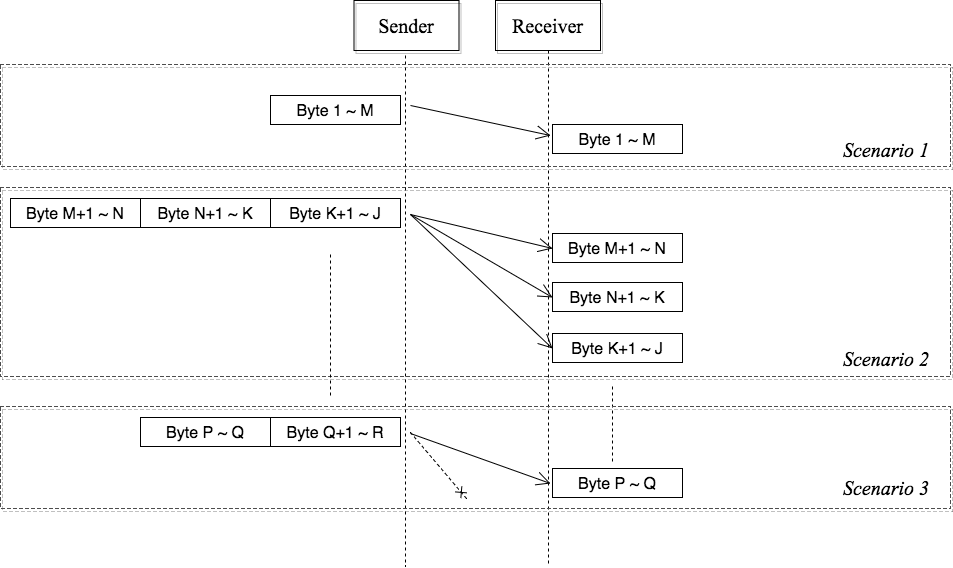
\includegraphics[scale=0.4]{Figures/namedpipe}}
\caption{Data transfer scenarios for Named Pipe}
\label{namedpipe}
\end{figure}

The content preservation verification is trivial. It compares the concatenation of the packet content of the sent events in a stream to the concatenation of the packet content of the receive events in the other stream, which is presented in Algorithm \ref{dataAlg1}. Since the concatenation needs to inspect the events in the streams, the time complexity of this algorithm is $O(N)$, $N$ is the total number of data transfer events in the two streams.

\begin{algorithm}[H]
\DontPrintSemicolon
\caption{{\bf Data Verification of Named Pipe} \label{dataAlg1}}
\tcc{$s_0$ and $s_1$ are two matched streams from $trace_0$ and $trace_1$. The output boolean $satisfied$ is true if the matched stream satisfy the content preservation of a communication.}
\KwIn{$s_0, s_1$}
\KwRet{$satisfied$}\;
$send_0 \leftarrow$ concatenation of the payload of send function call events in $s_0.ss$;\;
$send_1 \leftarrow$ concatenation of the payload of send function call events in $s_1.ss$;\;
$receive_0 \leftarrow$ concatenation of the payload of receive function call events in $s_0.sr$;\;
$receive_1 \leftarrow$ concatenation of the payload of receive function call events in $s_1.sr$;\;
\KwRet{$receive_1$ is prefix of $send_0$ AND $receive_0$ is prefix of $send_1$ }
\end{algorithm} 

\subsection{Data Verification Algorithm for TCP}
TCP is the most basic reliable transport method in computer networking. TCP provides reliable, ordered, and error-checked delivery of a stream of octets between applications running on hosts in an IP network. The TCP header contains the sequence number of the sending octets and the acknowledgement sequence this endpoint is expecting from the other endpoint(if ACK is set). The basic data transfer characteristics of TCP are:
\begin{itemize}
  \item Bytes received in order;
  \item No data lost (lost data will be re-transmitted);
  \item No data duplication;
  \item Bytes sent in packet and received in packet, no re-segmentation.
\end{itemize}

Based on these characteristics,  the data transfer scenarios of TCP can be exemplified in Figure \ref{tcp}.

\begin{figure}[H]
\centerline{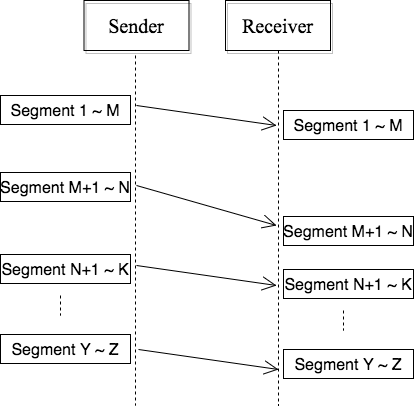
\includegraphics[scale=0.4]{Figures/tcp}}
 \caption{Data transfer scenarios for TCP}
\label{tcp}
\end{figure}

According to the data transfer properties of TCP, all packets sent in one side will be received in the same other in the other side. The verification can be restricted to packet to packet. If every $i-th$ send event in a stream can be matched by the $i-th$ receive event in the other stream for both directions, we can assert that the content preservation is satisfied for the communication. The verification algorithm of TCP is presented in Algorithm \ref{dataAlg2}. The time complexity of this algorithm is also $O(N)$, $N$ is the number of data transfer events in a stream.

\begin{algorithm}[H]
\DontPrintSemicolon
\caption{{\bf Data Verification of TCP} \label{dataAlg2}}
\tcc{$s_0$ and $s_1$ are two matched streams from $trace_0$ and $trace_1$. The output boolean $satisfied$ is true if the matched stream satisfy the content preservation of a communication.}
\KwIn{$s_0, s_1$}
\KwRet{$satisfied$}\;
\tcc{There is a chance that the trace capturing end before the channel is closed}
\For{$i \in {0..min(s_0.ss.size, s_1.sr.size)}$}{
     \If{$s_0.ss[i].payload\; \; != s_1.sr[i].payload$}{
       \KwRet False;\;
   }
}
\For{$i \in {0..min(s_1.ss.size, s_0.sr.size)}$}{
     \If{$s_1.ss[i].payload\; \;!= s_0.sr[i].payload$}{
       \KwRet False;\;
   }
}
 \KwRet True;\;
\end{algorithm} 


\subsection{Data Verification Algorithm for Message Queue}
Message Queue is a communication method to allow applications which are running at different times across heterogeneous networks and systems that may be temporarily offline to communicate with each other. Applications communicate to each other through the queue. Multiple sending applications can send messages to one queue and multiple receiving applications can read messages from one queue \cite{redkar2004pro}. In this work, only the case of one sending application versus one receiving application is considered. A queue can be one-way or duplex. The basic data transfer characteristics of Message Queue are:
\begin{itemize}
  \item Bytes sent in one packet are received in one packet, with no bytes re-segmented;
  \item Packets can be lost;
  \item Packets received in order;
  \item No data duplication.
\end{itemize}
Based on these characteristics, the data transfer scenarios of Message Queue can be exemplified in Figure \ref{msmq}.
\begin{figure}[H]
\centerline{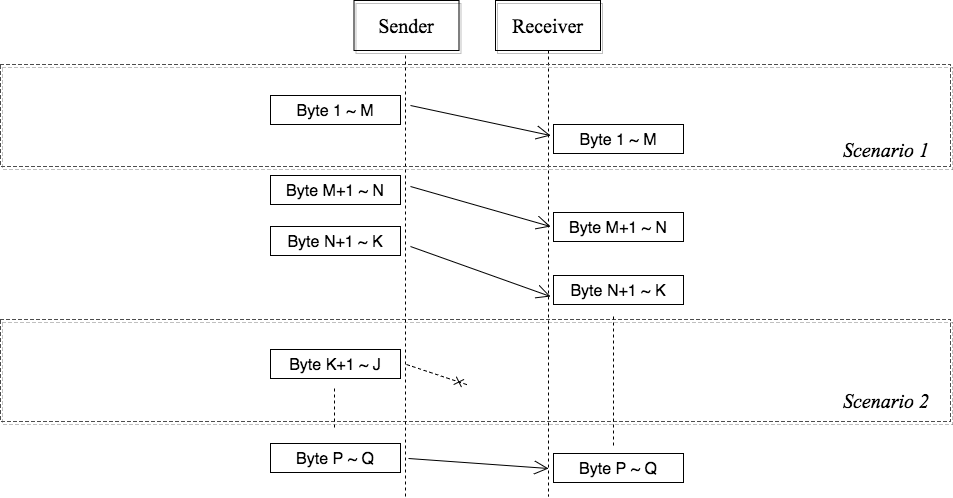
\includegraphics[scale=0.4]{Figures/msmq}}
\caption{Data transfer scenarios for Message Queue}
\label{msmq}
\end{figure}

To verify the content preservation of the unreliable communication, for each received packet, Algorithm \ref{dataAlg3} tries to find the matched sent packet in the other stream. If any of the received packets cannot be matched, the content preservation is not satisfied. Since the sent packets are received in order, the search for each received packet will start from the next index of the last matched sent packet. 

The time complexity of this algorithm is $O(N^2+M^2)$, $N$ and $M$ are the numbers of data sent events of the two streams.
\\
\begin{algorithm}[H]
\DontPrintSemicolon
\caption{{\bf Data Verification of Message Queue } \label{dataAlg3}}
\tcc{$s_0$ and $s_1$ are two matched streams from $trace_0$ and $trace_1$. The output boolean $satisfied$ is true if the matched stream satisfy the content preservation of a communication.}
\KwIn{$s_0, s_1$}
\KwRet{$satisfied$}\;
\If{$s_0.ss.size < s_1.sr.size$ Or $s_1.ss.size < s_0.sr.size$ }{
   \KwRet False;\;
}
$lastMatchIndex = 0$;\;
\For{$i \in {0..s_1.sr.size}$}{
     $tempIndex = lastMatchIndex$;\;
     \For{$j \in {lastMatchIndex+1..s_0.ss.size}$}{
             \If{$s_0.ss[j].payload = s_1[i].sr.payload$}{
                      $lastMatchIndex \leftarrow j$;\;
                      break the inner For loop;\;
            }  
     }   
\tcc{This received packet cannot be matched by any sent packet}    
     \If{$tempIndex = lastMatchIndex$}{
                      \KwRet False;\;
            }     
}     
$lastMatchIndex = 0$;\;
\For{$i \in {0..s_0.sr.size}$}{
     $tempIndex = lastMatchIndex$;\;
     \For{$j \in {lastMatchIndex+1..sends_1.size}$}{
             \If{$s_1.ss[j].payload = s_0[i].sr.payload$}{
                      $lastMatchIndex \leftarrow j$;\;
                      break the inner For loop;\;
            }  
     }   
     \If{$tempIndex = lastMatchIndex$}{
                      \KwRet False;\;
            }     
}  
 \KwRet True;\;
\end{algorithm} 

\subsection{Data Verification Algorithm for UDP}
UDP is a widely used unreliable transmission method in computer networking. It is a simple protocol mechanism, which has no guarantee of delivery, ordering, or duplicate protection. This transmission method is suitable for many real time systems. The basic data transfer characteristics of UDP are:
\begin{itemize}
  \item Bytes sent in packet and received in packet, no re-segmentation;
  \item Packets can be lost;
  \item Packets can be duplicated;
  \item Packets can arrive receiver out of order.
\end{itemize}

Based on these characteristics, the data transfer scenarios of UDP can be exemplified in Figure \ref{upd}.
\begin{figure}[H]
\centerline{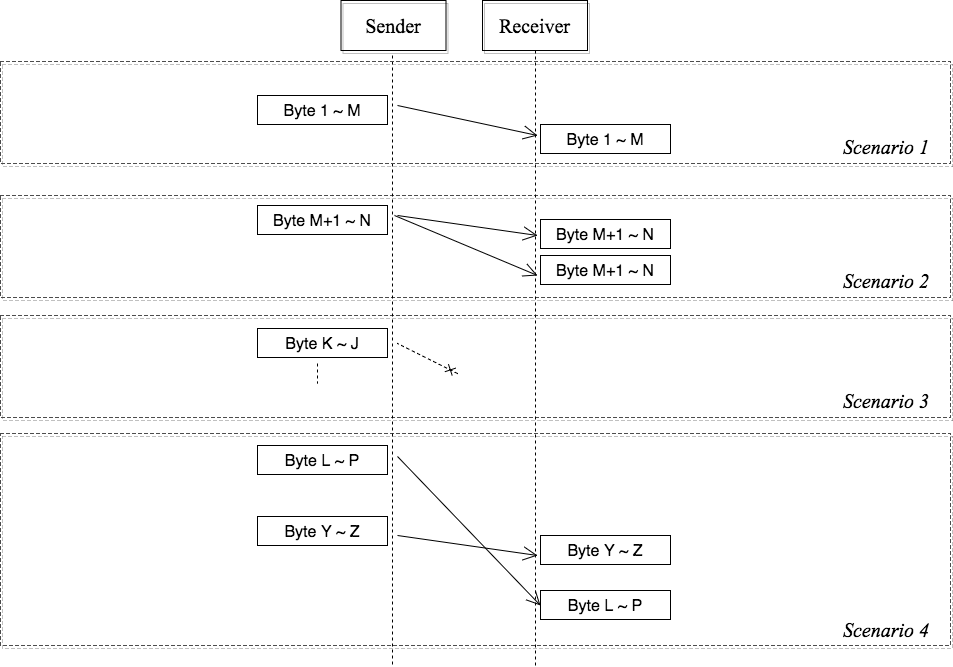
\includegraphics[scale=0.4]{Figures/udp}}
 \caption{Data transfer scenarios for UDP}
\label{upd}
\end{figure}

Similar to Message Queue, Algorithm \ref{dataAlg4} tries to match each received packet in one stream to the corresponding sent packet in the other stream. If any of the received packets cannot be matched, the content preservation is not satisfied. However, due to the potential reordering of packet, the matching is not restricted to the packet index (e.g, the $i-th$ received packet in one stream can be matched to the $j-th$ packet in the other stream, $i \neq j$). But the matched sent packet will be excluded from the following matching, which means each sent packet can only match to one received packet.

The time complexity of this algorithm is $O(N^2+M^2)$, $N$ and $M$ are the numbers of data sent transfer events in the two streams.
\\
\begin{algorithm}[H]
\DontPrintSemicolon
\caption{{\bf Transmitted Verification of UDP} \label{dataAlg4}}
\tcc{$s_0$ and $s_1$ are two matched streams from $trace_0$ and $trace_1$. The output boolean $satisfied$ is true if the matched stream satisfy the content preservation of a communication.}
\KwIn{$s_0, s_1$}
\KwRet{$satisfied$}\;
\If{$s_0.ss.size < s_1.sr.size$ Or $s_1.ss.size < s_0.sr.size$ }{
   \KwRet False;\;
}
\tcc{For each received packet in stream $s_1$ try to find the sent packet in stream $s_0$. $s_1.sr$ is the sequence of received packet of stream $s_1$ while $s_0.ss$ is the sequence of sent packet of stream $s_0$}
\For{$i \in {0..s_1.sr.size}$}{
    $matchFlag = False$;\;
     \For{$j \in {0..s_0.ss.size}$}{
             \If{$s_0[j].ss.payload = s_1[i].sr.payload$}{
                      $matchFlag = True$;\;
                      delete the packet from $sends_0$
                      break the inner For loop;\;
            }  
     }   
\tcc{This received packet cannot be matched by any sent packet}
     \If{$matchFlag = False$}{
                      \KwRet False;\;
            }     
}  
\tcc{For each received packet in stream $s_0$ try to find the sent packet in stream $s_1$. $s_0.sr$ is the sequence of received packet of stream $s_0$ while $s_1.ss$ is the sequence of sent packet of stream $s_1$}   
\For{$i \in {0..s_0.sr.size}$}{
    $matchFlag = False$;\;
     \For{$j \in {0..s_1.ss.size}$}{
             \If{$s_1[j].ss.payload = s_0[i].sr.payload$}{
                      $matchFlag = True$;\;
                      delete the packet from $s_0.ss$
                      break the inner For loop;\;
            }  
     }   
     \If{$matchFlag = False$}{
                      \KwRet False;\;
            }     
} 
 \KwRet True;\;
\end{algorithm} 

\subsection{Limitation of the Data Verification}
The verification discussed in this chapter has two major limitations:
\begin{itemize}
    \item The timing preservation of the communication is not verified.
    \item Some mismatching cannot be excluded even with the content verification
\end{itemize}  

The reason that the timing preservation cannot be verified is lacking timing information across the two traces. 

For the second limitation, the main reason is that the data transmitted in two communications could be identical or very similar. 

In Section \ref{streammatch}, I described how one stream in one side of the dual\_trace can be matched by two or more streams on the other side. In order to reduce this type of error, I developed the data verification strategy and algorithms. However, in some cases, the transferred data of two communications can be identical or very similar. Even with content verification, the mismatched streams still cannot be excluded.

Figure \ref{secondlevelmatching} exemplifies this situation in a reliable communication analysis. Assuming that $s_{11}$, $s_{21}$ and $s_{22}$ have the same channel identifier, they will be matched as two communications (one consists of $s_{11}$ and $s_{21}$ while the other one consists of $s_{11}$ and $s_{22}$). Furthermore, $s_{21}$ and $s_{22}$ send and receive the exact data. So both of the communications are considered to satisfy the content preservation property. In this case, the algorithms will not be able to determine if  $s_{11}$ communicated with $s_{21}$ or $s_{22}$. There is no way from the analysis point of view to distinguish the actual communication. It's more reasonable to preserve all of them in the output and present them for the users to make the decision. The users might be able to distinguish them and find the valid one.


\begin{figure}[H]
\centerline{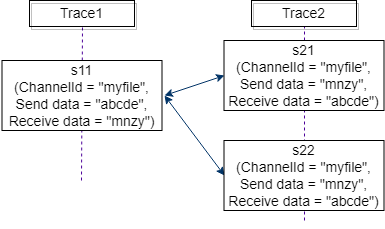
\includegraphics{Figures/secondlevelmatching}}
 \caption{An ineffective stream matching scenario}
\label{secondlevelmatching}
\end{figure}

\section{Discussion of Security Analysis Challenge}
Malware is a serious problem for all system nowadays. The intrusion of malware is generally an individual behavior, malwares attack the vulnerability of one or several specific systems, then intrudes into the system, destroys and controls it to obtains private information. Some malware can even be spread like a virus through the Internet, invading other systems with the same vulnerability. In general, malware is targeted at system-level intrusions, and there is very little damage to common application software unless there are obvious vulnerabilities that can be exploited for systematic attacks. \cite{leavitt2011mobile}

On the other hand, network attacks often occur on the network layer. Since the internet has be an extremely huge network in the world, the attack could be initiated at any network node. If there are no proper security measure, your data might be attacked during the transmission. There are many types of network attack, some are passive like monitoring information, some are active like corrupting and destroying the data or network itself. \cite{hansman2005taxonomy}

There is not a system that is absolutely secure from attackers. The running system's behaviour can change dramatically due to all of these attacks. The goal of the communication analysis is simply monitoring
programs in terms of data transmission. Perhaps the communication is modified by the attacks mention above. This places a huge challenge for communication analysis. For example, the identification of  a modified communication would be an extremely difficult mission. 

However, even though there might be some cases that the communication can not be effectively identified, this work will still be valuable to the analyst, as it will show that the data sent was not received (at least the same data was not received) by the other side and might mean that the running environment is compromised.

